%% Maybe mention the difference between regression and classification problems
\glsreset{GAN}

\chapter{Machine Learning and Neural networks} \label{cha:neuralNets}

Machine learning is the discipline of computer science where the goal, instead of laying down the steps for a machine to produce a result given some inputs, is in fact to make the machine find by itself (``learn'') the correct course of action by showing it relevant data. A more rigorous definition is given by \textcite{machineLearning1997}.
\begin{citacao}
    A computer program is said to learn from experience E with respect to some class of tasks T and performance measure P, if its performance at task T, as measured by P, improves with experience E. \cite[p. 2]{machineLearning1997}
\end{citacao}

In this definition the experience E can be viewed as the data that is used to teach the machine \textbf{--} this could be for example a dataset of images that the computer is expected to classify with the correct label (see \autoref{sub:supervised_learning}), or also repeated self play to become better at games like chess or Go as seen in reinforcement learning (see \autoref{sub:semi-supervised_and_RL}), where AlphaZero is a notable example \cite{alphaZero2017}.
The task T is what the machine is ultimately trying to achieve (e.g. classify images, play chess) and P is the measure of success in the task (e.g. percentage of accurately classified images, proportion of wins against an opponent in chess).

There are multiple approaches that fall unto the category of machine learning, popular techniques include \gls{KNN}, decision trees, random forest, \gls{SVM}, linear and logistic regression, and others\footnote{
    The paper from \textcite{fashionMNIST2017} gives many performance results for different methods applied on the Fashion MNIST dataset
}. Among the existing methods, neural networks have shown very good results in the last years, specially after the resurgence of deep learning thanks to the increased computational power, better use of parallelization, and the development of frameworks like Pytorch and Tensorflow.

Currently, neural networks are at the forefront of many areas like image classification\footnote{
    Big breakthrough in 2012 with AlexNet and the resurgence of Convolutional Neural Networks \cite{alexnet2012}
}, reinforcement learning\footnote{
    AlphaGo was the first ever computer to be able to defeat a human professional player at the game of Go \cite{alphaGo2016} and it's successor AlphaZero was able to surpass it by learning entirely through self-play \cite{alphaZero2017}
}, and generative modeling; where \acp{GAN}, which are the main focus of this document, are showing very good results.

This chapter will explain what are neural networks and how they can learn by themselves, this learning process is also often called training. First however, it is worth to have a brief description of the different types of learning.


\section{Types of Machine Learning}
For a machine to learn it is necessary to have something for it to learn, some set of data that can point it to the desired behaviour. Depending on the type of data available it is possible to divide learning into 4 different categories: Supervised; Unsupervised; Semi-supervised; and Reinforcement Learning.

\subsection{Supervised Learning} \label{sub:supervised_learning}
The simplest way to teach a computer is to train it with both the input data and the expected output. For example, suppose a classifier that is trained on the \gls{MNIST} dataset, the goal of this classifier is to take a gray-scale image as input and return the corresponding digit as output. Since \gls{MNIST} also contains the labels, the training would consist of feeding the images to the learning algorithm and comparing the predicted digits with those given by the labels. The difference between the prediction and the real output can then be used to adjust the classifier in order to make future predictions more likely to be correct.

Learning problems where the data contains both the input and the desired output are known as Supervised Learning problems, this is currently the most common form of learning. The advantage of this approach is that it makes very explicit to the computer what is expected from it, resulting in generally easier learning when compared to other forms of learning that have incomplete data.

The biggest problem with supervised learning is producing the datasets in the first place, obtaining the input data is generally simple, however producing the corresponding outputs (e.g. labels for classification problems) can be very difficult. For problems like image colorization \cite{colorization2016} or super resolution \cite{ganSuperResolution2016} this is trivial (i.e. convert a colorized image to gray-scale, downscale high resolution images), however for a dataset like \gls{MNIST} it is necessary to have a human label every single one of the $70,000$ images. For bigger datasets like ImageNet \cite{imageNet2015} that contain millions of images, classified into thousands of different classes, and that have annotated bounding boxes for a significant number of the images, the process is very slow and expensive. Amazon Mechanical Turk 
\footnote{
    Mechanical Turk page: \url{https://www.mturk.com}
}%
is often used for such tasks.

\subsection{Unsupervised Learning} \label{sub:unsupervised_learning}
In contrast with supervised learning where all the data is often costly labelled, unsupervised learning refers to problems where only the input data is available and the network has no explicit notion of the desired outputs. These types of problems have a huge potential since the amount of unlabeled data is much larger, however, learning without labels is also much more difficult and it is still an active area of research.

Situations where unsupervised learning can be used are more rare and may require some specific prior knowledge of the datasets to work properly. The \gls{MNIST} dataset can be used again as a simple example to understand how this type of learning works. Suppose that it is desired to build a classifier for handwritten digits, but the only dataset available is \gls{MNIST} stripped of it's labels; it may seem impossible to learn anything from this since all the machine sees are just images without any notion of right or wrong classification.

The trick is to exploit the prior knowledge of the problem and the distributions of the dataset in order to make progress. Since the objective is to build a digit classifier, then one prior information is that the number of possible classes will be 10, or 11 if a class ``Not a digit'' is also included.

Also consider the size of the input space, for \gls{MNIST} this is a $28{\times}28 = 784$ dimensional space, and with gray-scale images the number of different possible inputs is $256^{28\cdot28} = 2^{6,272} \approx 10^{1888}$. In such high dimensional spaces, all of the sensible inputs (e.g. images of digits) are just a tiny fraction of the whole input volume. This holds true for basically all situations, any random sample from an input space (pixel values, letters, audio amplitude) will almost always fail to produce the structured data present in the real world (pictures, words and phrases, human voice) \cite[chap. 5]{deepLearningBook2016} \textbf{--} it can be said that real life data is \textit{sparse} on the input space.

Along with sparsity, real data is also not evenly spaced on these high dimensional spaces, but it is instead concentrated around a relatively small number of clusters. \textcite[chap. 5]{deepLearningBook2016} argue this point by noting that it is possible to take similar images and apply some transformations, like moving objects or changing the light, in order to move from one image to another in the cluster. For example, one could take an image of the number 0 in \gls{MNIST}, add some slight rotations or change the width of the strokes, and end up with a different image that still represented the number 0. However a transformation from the number 0 to the number 3 does not seem to be so simple, so at least in an intuitive sense this example gives an idea of why the sparse data is also clustered around some points.

Using this knowledge of clusters and the number of classes expected in a problem like \gls{MNIST}, one can build an algorithm like \gls{KNN} to divide the input space into a desired number of regions, using a measure of similarity between inputs from the dataset as a guide for the divisions. Without using any labels the resulting algorithm is able to tell in which of the regions a given input belongs. For the \gls{MNIST} case, these regions have strong correlation with the corresponding digit \textbf{--} \cite{fashionMNIST2017} obtained accuracies of above 95\% with this technique.

Of course this approach is very dependent of the dataset and type of problem, it is not always that unsupervised learning will be so straight forward or that the divided regions will correlate well with the desired output.

\acp{GAN}, the main focus of this document, are also primarily unsupervised learning approaches. In \autoref{cha:gans} it will be discussed in detail how they work and learn from the underlying data distribution.

\subsection{Semi-supervised and Reinforcement Learning} \label{sub:semi-supervised_and_RL}
Semi-supervised learning is an intermediate between fully supervised and unsupervised learning, it concerns situations where the dataset is only partially labeled, the idea behind it is to use the vast amounts of unlabelled data to support the training from the relatively small number of labeled data. Since unlabeled data is much more easily available, semi-supervised learning has a lot of potential for building better models by fully leveraging the available data \cite{semi_supervised2005}.

Reinforcement learning is particularly different from the other types of learning, it's objective is to teach an agent to interact with a changing environment; learning does not occur with a dataset, but is instead achieved through trial-and-error where the agent is rewarded or punished depending on it's actions \cite{reinforcement_learning1996}. AlphaZero is an example of a reinforcement learning agent, it learned to play chess, shogi, and Go entirely through self-play \cite{alphaZero2017}.

\section{Artificial Neural Networks}
To understand neural networks, first it is necessary to understand it's building blocks, artificial neurons. Commonly called just neurons, nodes, or units (the preferred term used in this document will be unit), these were historically inspired by biological neurons. The idea behind them is that a single unit is a very simple element that receives some inputs and produces an output, the real power comes from connecting many of these together, from thousands, to millions, or even billions of connections\footnote{
  As of writing this document GPT-3 is the biggest neural network model of all time, having 175 billion parameters \cite{gpt3_2020}.
}.
\begin{figure}[hbt]
    \centering
    \caption{Single unit representation}
    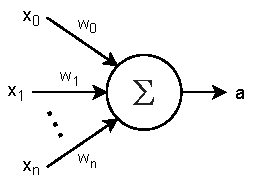
\includegraphics[width=0.4\textwidth]{chapters/NeuralNets/figures/neuron.pdf}
    \fonte{From the author (2021)}
    \label{fig:neuron}
\end{figure}

\autoref{fig:neuron} shows a representation of an artificial unit, it receives a set of inputs $[x_0, x_1, ..., x_n]$, denoted as a vector $\bm{x}$, and each input has a corresponding scalar value $w_i$ called it's weight. Units will also often have a bias term $b$ that is independent of the inputs and that is useful for shifting the output.

By changing the set of weights (in vector form $\bm{w}$) and the bias term, it is possible to achieve different behaviours from the unit based on it's inputs. \autoref{eq:weighted_input} shows how these parameters are used to calculate what is called the \textit{weighted input} ($z$) of the unit \cite[Chapter 2]{NN&DL2015}.
\begin{equation} \label{eq:weighted_input}
    z = \sum_{i}^{n}{w_i x_i} + b =
    %
    \begin{bmatrix}w_0, & w_1, & ... & w_n\end{bmatrix}^T
    \begin{bmatrix}x_0, & x_1, & ... & x_n\end{bmatrix} + b =
    %
    \bm{w}^T \cdot \bm{x} + b
\end{equation}

The weighted input is usually passed through a non-linear function $f$, called the \textit{activation function}, to produce the output $a$, called the unit activation, as seen in \autoref{eq:activation}.
\begin{equation} \label{eq:activation}
    a = f\left(z\right) = f\left(\bm{w}^T \cdot \bm{x} + b\right)
\end{equation}

A neural network is built by combining multiple units together and the learning process consists of adjusting all the weights and biases in order to produce the expected results given the dataset. Any combination of connections can be considered a neural network, however for the overwhelming majority of cases the networks are divided into layers, and for most of these cases the connections form an acyclic graph. This means that there are no cycles in the network, the input flows from one layer to the next, and there is usually no connection between layers that are not consecutive \textbf{--} exceptions to this are \gls{LSTM} networks \cite{lstm1997} and Residual Networks \cite{resnet2015}, but they are not the focus of this document.

The layers of the network are commonly divided into input layer, hidden layers, and output layer. The input layer represents the input data, usually in diagram representations the inputs are drawn like units, this however is just an stylistic choice since the values do not pass through any calculation in this layer.

The output layer contains the units that will be interpreted as the result produced from the input. For example, in a case where the network is trying to predict the price of apartments given area, number of rooms, and others properties (classical machine learning example), the output would be a single unit whose activation is the predicted price. Problems where the output can assume a range of values are usually called \textit{regression} problems.

On the other hand, problems where the output is better interpreted as a discrete value are called \textit{classification} problems. Predicting the digits of \gls{MNIST} falls into the category of classification problems, where the output represents which of the 10 possible digits the input image represents.

In the case of \gls{MNIST} the output layer can be made of 10 units, where each of the activations gives the probability of the input belonging to the corresponding digit. A natural question to raise from this description is: why would there be a need for one unit to represent each class, when the number 10 can be more efficiently represented using only 4 bits (4 units)? Or even, why not use just one unit that outputs the predicted number?

One reason for this is that these simpler representations would lose the property of interpretability of the output as a probability distribution. But the most important reason can be validated empirically, it is easier for a network to classify the inputs into isolated units then it is to try and correlate them with specific bits for each class \cite[Chapter 1]{NN&DL2015} or to reduce the output into a single unit.

For most classification problems using a neural network the output layer will contain one unit for each possible class and the desired output will be a vector where all elements are 0's, except for the element corresponding to the true label that will be a 1, indicating the 100\% probability for that class. This way of encoding the outputs is called \textit{one-hot encoding}.


The rest of the layers in a neural network, called the hidden layers, are all the layers between the input and output. A neural network does not need to have any hidden layers, but they are fundamental for building more complex relations and robust models.

\textcite{universalApproximator1989} showed that, given sufficient hidden units, any neural network with a single hidden layer can be used to approximate any function to any amount of precision, in other words, neural networks with at least a hidden layer are \textit{universal approximators}. But in practice it is observed that more hidden layers usually perform better, they are able to divide the problems into steps and gradually reach the result. For example, an image classifier might use the first layers to distinguish lower level features like edges, while deeper layers recognize shapes, textures, and all the way to complex patterns like faces \cite{deepLearningBook2016}.

More recent years have seen a resurgence of \gls{DL}, this is generally understood as learning with networks having at least two hidden layers, but modern models can have much more than that\footnote{
    Google's Inception v3 image classifier model has 42 layers in total \cite{inceptionV3_2015}
}.

\autoref{fig:network} shows an example of the layered structure of a neural network, for simplicity the diagram shows only fully connected layers (all the units of a layer are connected to all the units of the previous layer, see \autoref{subsub:fully_connected}) but it could also have different types of layer without losing the general idea of input, hidden, and output.
\begin{figure}[hbt]
    \centering
    \caption{Diagram of a fully connected neural network}
    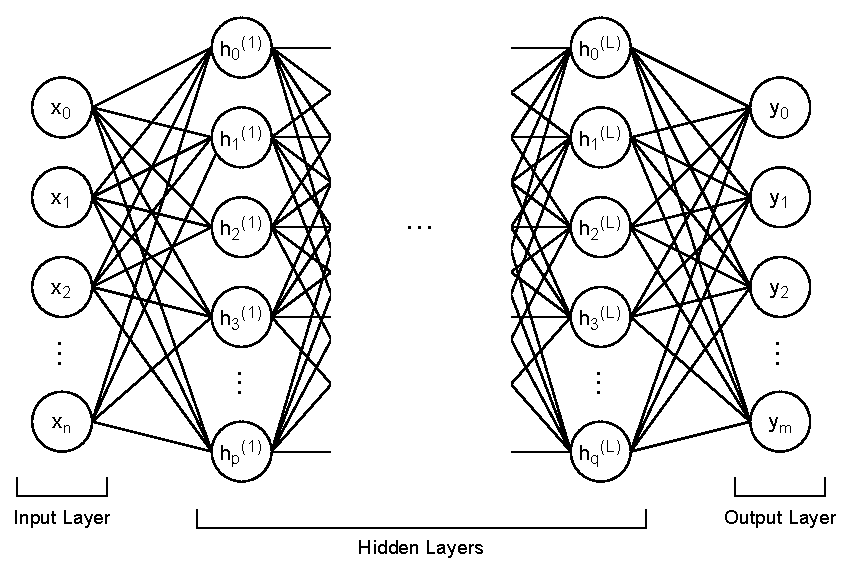
\includegraphics[width=0.8\textwidth]{chapters/NeuralNets/figures/network.pdf}
    \fonte{From the author (2021)}
    \label{fig:network}
\end{figure}


\subsection{Types of layers}
The networks constructed for this document will all use a combination of fully connected and convolutional layers. This section will explain how these work, how they differ, and their advantages in relation to each other.

Before proceeding however, it is important to define the notation that will be used. Since from now on the focus will changes from single units to an entire network, it is necessary to establish a notation that allows for indexing individual units, in any layer, and also their parameters.

The bias, weighted input, and activation for unit $i$ in layer $l$ will be written as $b_{i}^{(l)}$, $z_{i}^{(l)}$, and $a_{i}^{(l)}$ respectively. The weight connecting unit $j$ in layer $l-1$, to unit $i$ in layer $l$ will be written as $w_{ij}^{(l)}$.

The set of biases, weighted inputs, and activations in layer $l$ can also be written as the vectors $\bm{b}^{(l)}$, $\bm{z}^{(l)}$ and $\bm{a}^{(l)}$. The weights connecting the units in layer $l-1$ to units in layer $l$ can be written as the weight matrix $\bm{W}^{(l)}$.
\begin{equation*}
    \renewcommand{\arraystretch}{1.4}
    \setlength\arraycolsep{4pt}
    \bm{z}^{(l)} = \begin{bmatrix}
        z_{0}^{(l)} \\
        z_{1}^{(l)} \\
        \vdots \\
        z_{n}^{(l)}
    \end{bmatrix}
    %
    \quad
    \bm{a}^{(l)} = \begin{bmatrix}
        a_{0}^{(l)} \\
        a_{1}^{(l)} \\
        \vdots \\
        a_{n}^{(l)}
    \end{bmatrix}
    %
    \quad
    \bm{b}^{(l)} = \begin{bmatrix}
        b_{0}^{(l)} \\
        b_{1}^{(l)} \\
        \vdots \\
        b_{n}^{(l)}
    \end{bmatrix}
    %
    \quad
    \bm{W}^{(l)} = \begin{bmatrix}
        w_{00}^{(l)} & w_{01}^{(l)} & \dots  & w_{0m}^{(l)} \\
        w_{10}^{(l)} & w_{11}^{(l)} & \dots  & w_{1m}^{(l)} \\
        \vdots       & \vdots       & \ddots & \vdots \\
        w_{n0}^{(l)} & w_{n1}^{(l)} & \dots  & w_{nm}^{(l)}
    \end{bmatrix}
\end{equation*}

Recall that the activation of a unit is simply it's activation function, denoted here as $f$, applied to the weighted input. \autoref{eq:activation_again} rewrites this relation as shown in \autoref{eq:activation} using the revised notation.
\begin{equation} \label{eq:activation_again}
    \bm{a}^{(l)} = f\left( \bm{z}^{(l)} \right)
\end{equation}

Observe that in \autoref{eq:activation_again} the activation function is applied to the vector $\bm{z}^{(l)}$, this is a common shorthand notation to represent the element-wise application of the function to the vector. This notation will be used throughout the entirety of this document, all functions applied to vectors will be applied element-wise unless otherwise noted.

\subsubsection{Fully connected layer} \label{subsub:fully_connected}
Fully connected, also called Dense layers, are a type of layer where all the inputs are connected to all outputs of the previous layer. \autoref{eq:dense_weighted_input} shows how the weighted inputs of this layer are calculated from the activations of the previous layer.
\begin{equation} \label{eq:dense_weighted_input}
    z_{i}^{(l)} = \sum_{j}{w_{ij}^{(l)} a_{j}^{(l-1)}} + b_i^{(l)}
\end{equation}

If the previous layer is the input layer, the values for $\bm{a}^{(l-1)}$ will be the input of the network. To abstract the type of input it is useful to just replace the notation with a general layer input $\bm{x}$. The activation can be written more simply by using vector form as shown in \autoref{eq:dense_activation}, the layer superscripts were also omitted for more clarity.
\begin{equation} \label{eq:dense_activation}
    \bm{a} = f\left( \bm{W}\bm{x} + \bm{b} \right)
\end{equation}

Dense layers are extremely common, being used in many types of neural networks. They are very useful for mapping their inputs, that can have any number of dimensions, to a vector with any different number of dimensions, this is used in almost all classifiers to reduce the detected features into a one-hot encoded vector of the possible classes. For example, in the 2012 ImageNet challenge the three last layers of the network AlexNet were fully connected, they mapped the $43,264$ features into a $1000$ dimensional vector corresponding to all classes of images in the challenge \cite{alexnet2012}.

This type of layer can also be used to apply transformations to features that will be used later in the network, this is used in \acp{GAN} to map the latent space to a vector that is transformed into the generated image (see\autoref{cha:gans}). They can even be used for full feature extraction, but this is usually not the best choice since they are quite expensive given the high number of connections and, as will be seen, they lack some useful properties that are present in convolutional layers.


\subsubsection{Convolutional layer}
One drawback of fully connected layers is that they do not leverage the structure of the data when calculating the activations. Consider for example the case of images, when dealing with random values all pixels are uncorrelated with one another, but in real world situations the pixels of an image group together to make edges, shapes and complex figures. The same could be said for audio, video, language and many other situations \cite{guide_conv2018}.

Consider the example of a simple image of a digit in the \gls{MNIST} dataset, by translating the image by a couple of pixels or by slightly warping the strokes the digit represented does not change. But since the fully connected layer has no sense of neighbouring pixels (or temporal coherence for audio and video, etc.), then it has no choice other than learning weights for all possible slight transformations to the inputs. This not only makes learning more difficult, but also introduces many unnecessary parameters to the network.

Convolutional layers are a way of dealing with this problem. Initially inspired by the visual cortex of vertebrates \cite{neurocognitron1982}, the idea behind them is to detect the presence of features, no matter where they are present or if they are slight perturbed (e.g. an edge should be seen as an edge, no matter where it is located in the image or if it is slightly rotated).

Neural networks that employ convolutional layers are usually called \acp{CNN}, their history is very long and they were already used in the 1990's for learning the \gls{MNIST} dataset when it was introduced \cite{mnist1998}. However they were not very popular for larger problems and only grew in popularity after the great breakthrough in the ImageNet challenge achieved by the \gls{CNN} AlexNet in 2012 \cite{alexnet2012}. Since then they have become very common and are used in a variety of situations, even outside of image recognition. 

This section will only explain how they work for the 2-dimensional case, but the idea can be easily generalized to the 1-dimensional or multidimensional cases. The inputs of a convolutional layer share the properties that they are represented as multidimensional arrays, have one or more axis where the ordering matters (for images these are the width and height), and can have an axis representing different views of the data (e.g. the RGB channels for a colored image) \cite{guide_conv2018}.

The name convolution is not a coincidence, the layer operation is related to the convolutions seen in signal processing for 1D discrete signals, the image convolutions like gaussian and Sobel filters, or higher dimensions mathematical convolutions. The operation consists of sliding a window of weights, called the kernel, over the entire input and calculating the sum of the weighted inputs covered by this window to produce the resulting values.
\begin{figure}[hbt]
    \centering
    \caption{Convolutional layer kernel properties}
    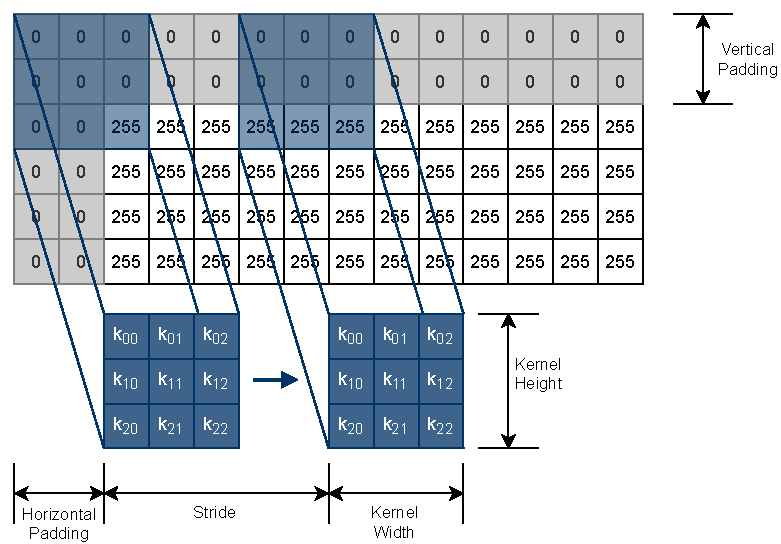
\includegraphics[width=0.55\textwidth]{chapters/NeuralNets/figures/cnn.pdf}
    \fonte{From the author (2021)}
    \label{fig:kernel_properties}
\end{figure}

It is simpler to understand this by looking at an image representation, \autoref{fig:kernel_properties} shows an example of a kernel being applied at the corner of an image with a single channel, whose values are $255$, and that is padded with zeros.

As seen in the figure, the kernel will start at the top left of the image (including some optional zero padding) and calculate a value for that position, then it will step a number of pixels, called the stride, and calculate the next value. When there is no more room to step horizontally, the kernel will start again at the left of the image and step a stride size downward, this is repeated until the whole image is traversed.

The convolution value between the kernel window and the pixels is simply the sum of the element wise products between the pixel values and the corresponding kernel weight. An image can be used again to help visualize this process, \autoref{fig:convolution} shows how a convolution is calculated for a $3\times3$ kernel, on a $3\times3$ image, with $1$ pixel zero padding, and stride of $1$ for both horizontal and vertical directions.
\begin{figure}[hbt]
    \centering
    \caption{Simple convolution process}
    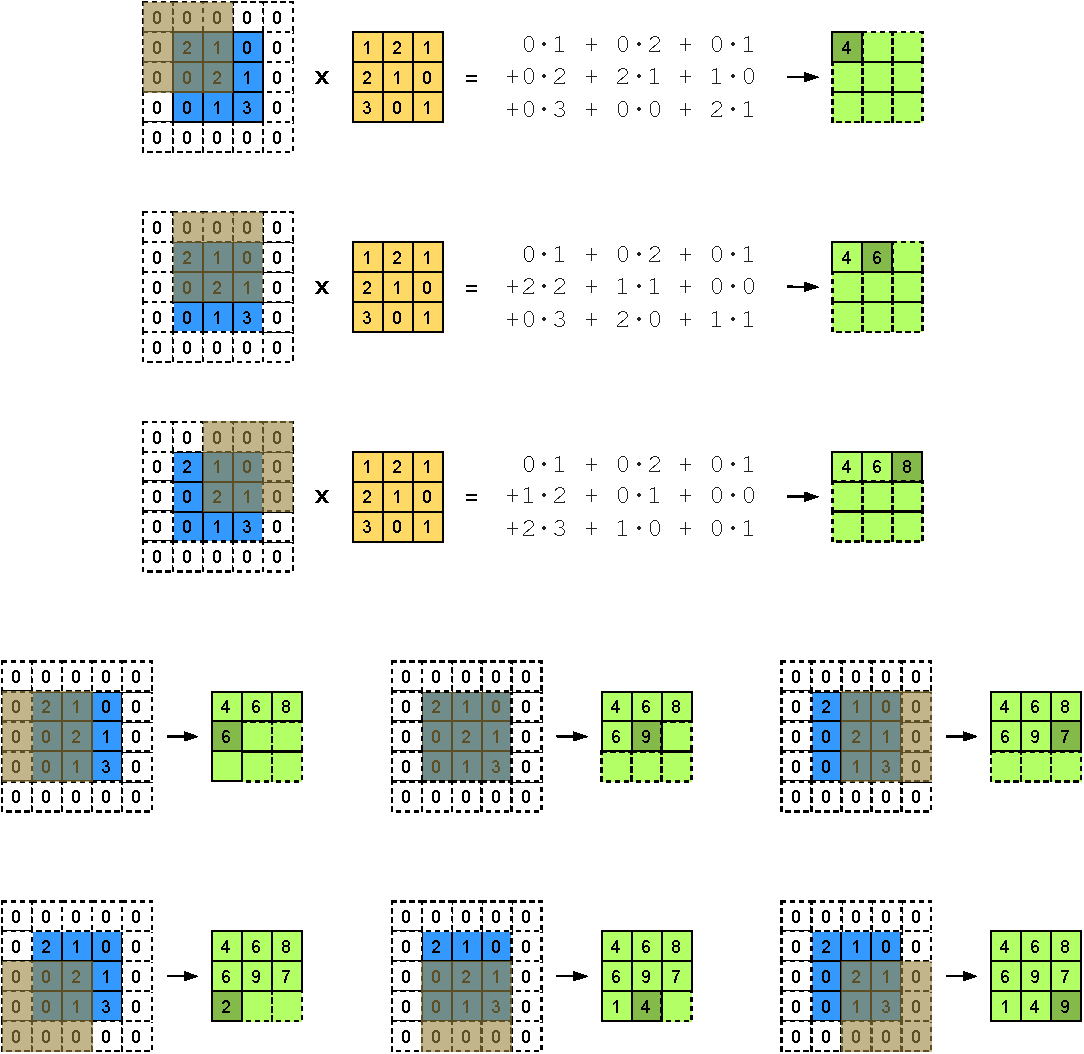
\includegraphics[width=0.7\textwidth]{chapters/NeuralNets/figures/convolution.pdf}
    \fonte{From the author (2021)}
    \label{fig:convolution}
\end{figure}

Also note that the kernel does not change when calculating the outputs of the convolution, in other words, the weights of the kernel are shared between the units. These weight are learned instead of being predefined, this allows for the network to decide which features the kernels should detect in order to solve the problem; these could be for example edges, textures, shapes, specific colors or others.

One important detail to mention is that the examples shown until now only consist of single channel images. For colored images with 3 channels, and more general cases with $n$ channels, the kernel is not just a 2D matrix but is more accurately represented as a volume (i.e. one 2D kernel for each channel) . This means that in \autoref{fig:convolution} the kernel is a $3\times3\times1$ volume, if the input were a colored image it would be a $3\times3\times3$ volume. For the general case of an $n$ channel input, the volume would be $h\times w\times n$ for a kernel with height $h$ and width $w$.

The convolution for multiple channels is basically the same as for a single channel, each $h\times w$ slice of the volume is convoluted with one of the channels and the results are added together to get the final convolution. These resulting values can be considered as the weighted inputs $\bm{z}$ of the convolutional layer, so the activation function should be applied in order to get the final layer output.

In summary, for the case of images, a convolutional layer takes as input a 3D volume (i.e. two spatial dimensions to convolve with, and 1 channel dimension to give different views of the image) and operates on it using a kernel volume, the spatial sizes of the kernel are free to choose, but the number of channels must match. The convolution operation with a single kernel will reduce the input volume to a 2D feature map, where each point in the map indicates how much the feature is present at that region of the input covered by the kernel window. In general it is desirable to detect many different features from the input image, this means that convolutional layers will have multiple kernels and all the resulting convolutions will be stacked to produce an output volume.

The output will have as many channels as the number of kernels used in the convolutional layer, but the width and height will depend on the kernel size, stride, and padding. Consider sliding the kernel in the horizontal direction (the same logic applies to any direction and for all input dimensions), the number of values calculated by the convolution will be the number of possible positions that the kernel can be placed in this direction.

Suppose that in the horizontal direction the sizes of input, kernel, zero padding, and stride are $i$, $k$, $p$, and $s$ respectively. Then the output size $o$ in this direction is given by \autoref{eq:conv_output_size} \cite{guide_conv2018}, where $\lfloor{.}\rfloor$ is the floor function.
\begin{equation} \label{eq:conv_output_size}
    o = \left\lfloor{
        \frac{i + 2p - k}{s}
    }\right\rfloor + 1
\end{equation}

Convolutions can be used to enlarge the input image, but are most commonly used to reduce the dimensions while raising the number of features detected. For example, the GoogLeNet Inception architecture reduces the $224\times224\times3$ input image to a feature map of size $7\times7\times1024$ \cite{inceptionV1_2014}. This reduction is usually not done using only a single convolutional layer, it is most common for the input volume to pass through multiple convolutions that gradually reduce it's width and height while increasing it's depth. Looking at the Inception model again, the whole network is $22$ layers deep with most of those being convolutions for feature extraction \cite{inceptionV1_2014}.

According to \textcite[chap. 9]{deepLearningBook2016}, convolutional layers leverage the ideas of sparse interactions, shared parameters, and equivariant representations to improve a machine learning system. They describe sparse interactions in the sense that kernels are smaller than the input, reducing the number of parameters, the memory used, the processing cost, and improving statistical efficiency. And the idea of equivariant representations is related with the invariance to translation, since at least in principle, the use of a sliding window allows for detecting the same feature no matter where it might appear on the image.

\subsubsection{Transposed Convolutions}
Any convolution operation can be converted to a matrix multiplication where the input is flattened to a 1-dimensional vector and the kernel is converted to a sparse matrix $\bm{C}$. The forward pass through the network, which is when the convolution is applied, is equivalent to multiplying the flattened input by $\bm{C}$, and the backward pass is equivalent with multiplying by $\bm{C}^T$ \cite{guide_conv2018}. The multiplication with $\bm{C}^T$ converts the output volume to the input volume and is commonly called the transposed convolution, or sometimes \textit{deconvolution}.

Any kernel represents both a convolution or transposed convolution, it all depends on how the values are interpreted as a matrix. It is important to note that the transposed convolution is not a way to reverse the convolution step, it is generally not possible to calculate the input of a convolution based on the kernel and output values. But the transpose operation can be considered as a reverse in the sense of transforming the output volume into the input volume.

Given the property of producing the opposite volume in relation to convolutions, transposed convolution layers are commonly used to upscale data to higher dimensions. For example, they are used in \acp{GAN} to upscale the latent space vector into the corresponding image (see\autoref{cha:gans}) \cite{nipsGAN2017}. However, upscaling with this method has been shown to produce image artifacts \cite{deconvolutionArtifacts2016} and some models, like styleGAN \cite{styleGAN2018}, already drop the use of transposed convolution layers for different upscaling approaches.

\subsubsection{Pooling layer}
Pooling layers are very similar to convolutional layers in the sense that they both slide an window of some width and height through the image, using some stride value, optional padding, and producing a number for each possible position of the window. But pooling layers do not have any learnable parameters and just execute a predefined function over all the inputs inside the sliding window to produce the output.

The two most common types of pooling are max and average pooling. Max pooling, as the name suggests, simply returns the maximum value present in the sliding window, while average pooling returns the average of those values. Pooling layers are very commonly used together with convolutional layers, \textcite[p. 355-336]{deepLearningBook2016} describe that a usual convolutional layer in a \gls{CNN} consists of a convolution operation, followed by the nonlinear activation, and lastly by a pooling layer; they say that this operation helps to make the representation approximately invariant to input translations.

\subsubsection{Embedding Layer}
This layer is an alternative way of representing discrete valued inputs. Recall that one way to represent a discrete value (e.g. the class of a given input) is to use one-hot encoding, this allows for mapping $n$ possible values into a $n$ dimensional vector of all 0's and a single 1 representing the value.

Embedding layers offer a way to map $n$ values into a vector with $m$ dimensions, where $m$ can be any number. The mapping from value to vector in an embedding layer is not something fixed, but is also learned during training. This type of layer is very useful in language models, where encoding thousands of possible words into one-hot vectors is infeasible, embeddings allow for much smaller representations that can be learned by the model to best fit a given problem.

When conditioning \acp{GAN} with class information for the \glsunset{CGAN} \gls{CGAN} variant (see \autoref{sub:cgan}), it is necessary to combine the label of the data together with the input. Embedding layers offer a more robust solution to this when compared to one-hot vectors, because of that they were used for conditioning in the experiments seen in\autoref{cha:experiments}.


\subsection{Activation Functions}
Historically one of the first implementations of artificial neural networks used the step function as activation for the units \cite[Chapter 1]{NN&DL2015}, this means that for positive inputs the step function produces a $1$ and for all other values it produces a $0$. It also could use the sign function \cite{thePerceptron2017}, producing a $-1$ for non positive inputs.

This type of approach is called a Perceptron, one notable example of it's implementation was the MARK I Perceptron, a hardware solution where all weights were regulated by potentiometers and automatically adjusted by motors to train the network \cite{perceptron1960}. However it was later shown that this type of binary activation was very limited and could only solve linear separable problems \cite{thePerceptron2017}.

One may question the need for activation functions or why do they need to be nonlinear, what is the reason for introducing nonlinearity to the network? To understand this, first note that not using an activation function is the same as setting the output $y = x$, this is also a linear relationship between the values, so it is only necessary to explain why a linear activation is a problem.

The nonlinearity is introduced to make the network able to learn more complex relationships in the data, since not all real world situations have a linear dependence between input and output. By transforming the input through multiple nonlinear activations it is possible to create very elaborate mappings from input to output. This does not hold true for linear transformations, since applying a sequence of them to some input is equivalent to applying just a single one.

To see this consider an input vector $\bm{x}$ with two transformations matrices $\bm{A}_1$, $\bm{A}_2$ and vectors $\bm{b}_1$, $\bm{b}_2$. The output $\bm{y}_2$ is obtained by applying two linear transformations to the input vector as follows.
\begin{equation} \label{eq:linearity_1}
    \bm{y}_1 = \bm{A}_1 \bm{x} + \bm{b}_1
    \qquad \text{and} \qquad
    \bm{y}_2 = \bm{A}_2 \bm{y}_1 + \bm{b}_2 \\
\end{equation}

By rearranging the terms it can be confirmed that the two linear transformations are equivalent to a single one, this can be seen by the following derivation.
\begin{align*}
    \bm{y}_2& = \bm{A}_2 (\bm{A}_1 \bm{x} + \bm{b}_1) + \bm{b}_2 \\
    & = \bm{A}_2 \bm{A}_1 \bm{x} +  \bm{A}_2 \bm{b}_1 + \bm{b}_2 \\
    & = \bm{A} \bm{x} + \bm{b}
\end{align*}

This logic holds true for any number of linear transformations. Now it should be hopefully clear to see that there is inherently no difference between a multilayered neural network with linear activations and a simple two layered input-output network. It is necessary to introduce nonlinearities in the hidden layers in order to build more complex models \textbf{--} linear transformations can however be used in the output layer to map the values to a more desirable range, regression problems are an example.

Although nonlinear, the binary property of the step function limits the capabilities of a neural network, to work around this limitations it is necessary to introduce a different type of activation. To avoid the problem of jumping values it is best to have a continuous function instead of a discrete one, it is also important that this function be differentiable in it's domain and that the derivatives are not zero everywhere (see \glsunset{ReLU} \gls{ReLU} activation in \autoref{subsub:relu} for more remarks about this restrictions). The derivative requirements are necessary to make possible the use of the learning algorithm Gradient Descent with Backpropagation (see sections \ref{sec:loss_&_gradient_descent} and \ref{sec:backpropagation}).

This section will briefly introduce some important activation functions that are widely used in multiple machine learning problems and that were used in the experiments found in\autoref{cha:experiments}.

\subsubsection{Sigmoid} \label{subsub:sigmoid}
Usually denoted by \gls{sigmoid}, the sigmoid function maps all real numbers to the interval $(0, 1)$. For a given input $x$, the value for $\sigma(x)$ is given by \autoref{eq:sigmoid}.
\begin{equation} \label{eq:sigmoid}
    \gls{sigmoid}(x) = \frac{1}{1 + e ^ {-x}}
\end{equation}

The sigmoid function can be considered the continuous version of the step function, as the absolute value of $x$ grows, $\sigma(x)$ gets exponentially closer to $\mathsf{step}(x)$, but there is a continuous transition close to $0$. This can be seen more clearly in\autoref{fig:activations}.
\begin{figure}[hbt]
    \centering
    \caption{Curves of sigmoid, tanh and ReLU activation functions}
    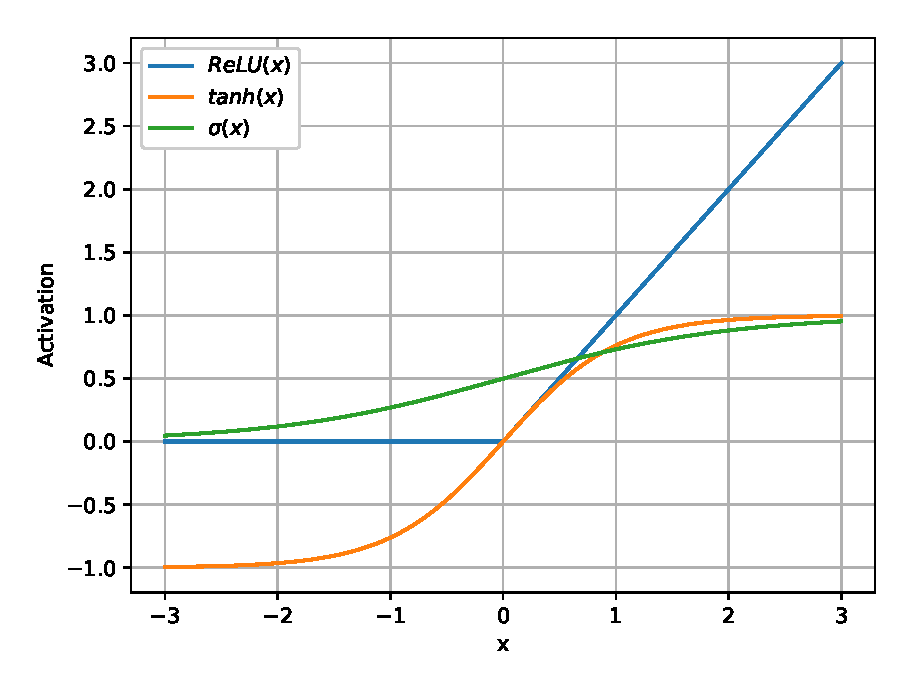
\includegraphics[width=0.6\textwidth]{chapters/NeuralNets/figures/Activations.pdf}
    \fonte{From the author(2021)}
    \label{fig:activations}
\end{figure}

This function can be useful to convert a single output to a probability value or to normalize a set of outputs. However, the fact that the outputs are always positive raises some problems, \textcite{efficientBackprop2012} showed that in these situations the backpropagation algorithm must update all the network parameters in the same direction, this means that the parameters are not free to wander the parameter space in the best direction.

Most of the time the network will benefit more by adding to some parameters while subtracting from others, the restriction to always update in the same direction makes learning more difficult and can greatly reduce the speed of convergence. \textcite{efficientBackprop2012} also argue that any deviation in the average of the outputs will bias the update direction, so it is better to have activations that are zero centered.

Knowing this problem, it only makes sense to consider sigmoid activations in the output layer, since for most cases it is better to use a zero centered alternative like the \gls{tanh} in the hidden layers.

\subsubsection{Hyperbolic Tangent}
The hyperbolic tangent function, as seen in \autoref{eq:tanh}, is a zero centered, scaled, and shifted version of the sigmoid function.
\begin{equation} \label{eq:tanh}
    \tanh(x) = \frac{e^x - e^{-x}}{e^x + e^{-x}} = 2\sigma(2x) - 1
\end{equation}

This function is almost always better than sigmoid since it has the same shape and properties without having the disadvantage of not being zero centered. It can be used in any layer, including the output. The times were a sigmoid would be preferred are when it is desired that the output be bounded to $(0,1)$, as is the case for a probability value.

\subsubsection{Rectified Linear Unit} \label{subsub:relu}
\glsreset{ReLU}
Both the sigmoid and hyperbolic tangent functions have two characteristics that can raise some problems when training a machine learning model. The first one is that they can only produce very close approximations of the number zero, but not the exact value \textbf{--} the only exception would be when the input of the \gls{tanh} function is also exactly zero, but this is very unlikely to happen and would only work for very specific inputs.

The lack of a true zero can be undesirable when the goal of the network is to build a sparse representation of the data, that is, a representation that only depends on a small number of inputs that strongly correlate to the output. This is in contrast with a model that depends on many inputs, but most of them have very little impact on the output.

The sparsity argument not only has some biological support, but has been shown to also positively influence the quality of a model \cite{relu2011}. Promoting sparsity is found in many other areas of science (e.g. statistical modeling, image compression) and it is very useful for producing simpler representations of the data \cite{dataDrivenScience2019}.

The other problem present in the sigmoid and \gls{tanh} functions is that they saturate for high absolute values of the input. Most of the variation in these functions occur close to zero, but for larger values there is barely any difference between outputs. For example, the difference between the \gls{tanh} activation between inputs $1$ and $2$ is around $0.2$, while the difference from $2$ to $100$ is just $0.036$. One other way to say this is that the derivatives of these functions are very close to zero for inputs far from the origin (see \autoref{fig:derivatives}), this can give rise to the vanishing gradients problem and make learning extremely slow (see \autoref{sub:vanishing_gradients}).
%
\begin{figure}[hbt]
    \centering
    \caption{Derivative of sigmoid, tanh and ReLU activation functions}
    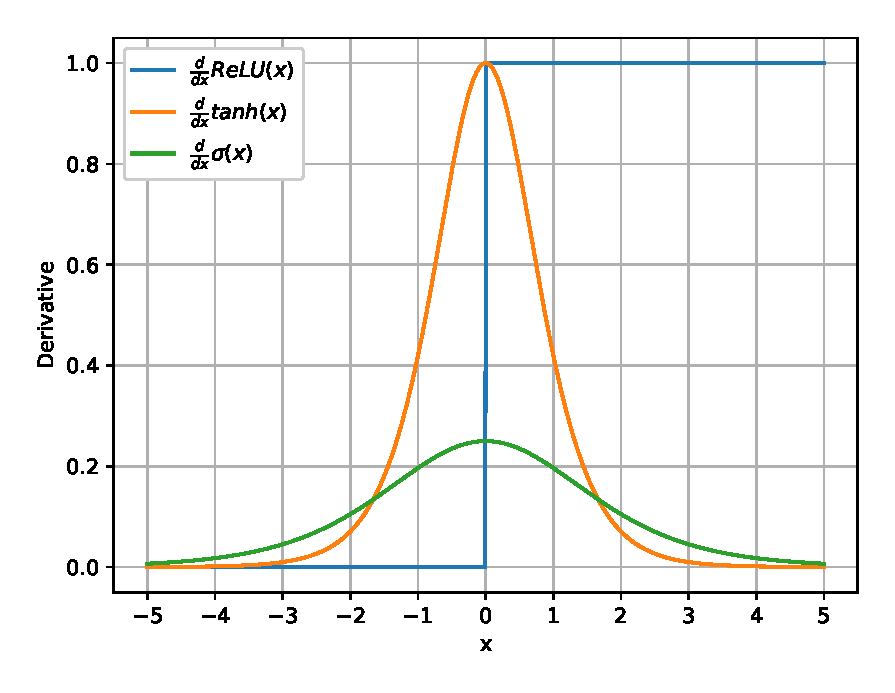
\includegraphics[width=0.6\textwidth]{chapters/NeuralNets/figures/Derivatives.pdf}
    \fonte{From the author(2021)}
    \label{fig:derivatives}
\end{figure}

The \gls{ReLU} activation function is an alternative that addresses both of the mentioned problems with sigmoid and \gls{tanh}. It is constructed from combining different linear regions (called a piecewise linear function), this allows for the activation to inherit many desirable properties of linear transformations while still retaining nonlinearity and being able to build complex relations \cite{deepLearningBook2016}.

The \gls{ReLU} function is simply composed of a constant zero for all negative inputs and the identity function for everything else, this means that for an input $x$ the activation is calculated as shown in \autoref{eq:relu}.
\begin{equation} \label{eq:relu}
    \ReLU(x) = \max(0, x)
\end{equation}

This definition allows for \gls{ReLU} to produce exact zeros for any negative inputs, promoting sparsity in the model representations. The constant positive derivative (see \autoref{fig:derivatives}) also removes the problem of vanishing gradients, since the units never saturate. Another big advantage of \gls{ReLU} is that it is extremely easy to compute, a simple \texttt{if} statement is enough to get the result; compared with the need to calculate exponentials in the sigmoid and \gls{tanh} functions, \gls{ReLU} performance is much faster.

Since around 2010, with papers like \cite{relu2011} exploring the \gls{ReLU} activation, there were many popular methods that showed impressive results using this function (e.g. \cite{alexnet2012} and \cite{inceptionV3_2015}). At the current time \gls{ReLU} is the standard recommended activation function to be used in most problems \cite{deepLearningBook2016}.

There are however some downsides to this activation. First there is the sharp change in the function behavior at the value $0$, making it's derivative undefined at that point, this however does not seem to be a problem in practice \cite{relu2011}. \gls{ReLU} also loses the desirable zero centered property that made \gls{tanh} a good substitute for the sigmoid, the argument from \textcite{efficientBackprop2012} holds for all activations, this means that all the network updates for units that use \gls{ReLU} must be made in the same direction, making learning more difficult.

Lastly, for a unit to be able to learn it is necessary that it outputs a value in the range where the activation function has a non-zero derivative for at least one example in the training data. But it is possible that for all the training data in a given problem, there exists some units using \gls{ReLU} activations that will always output zero, this makes learning impossible in these units and effectively freezes them on their state forever.

There are many other alternatives proposed to address these problems, some relevant examples are Maxout, LeakyReLU, ELU, GELU and PReLU, these have found some success in big machine learning problems\footnote{
    GELU is used in natural language processing models like GPT-3 \cite{gpt3_2020}
} and the benchmark by \cite{CaffeNetBench2017} showed good results for some of these alternatives \textbf{--} although \gls{ReLU} also fared well in those tests.

Between these alternatives, LeakyReLU is specially relevant for \acp{GAN}, being an important piece of the \glsunset{DCGAN}\gls{DCGAN} variant that is the base of many \gls{GAN} architectures. It consists of a simple change from ReLU that just guarantees that the units will always have at least some positive derivative. This activation is calculated as shown in \autoref{eq:leaky_relu}, where $\alpha$ is a hyperparameter that must be a small value (usually $0.3$).
\begin{equation} \label{eq:leaky_relu}
    \LeakyReLU(x) = \max(\alpha x, x)
\end{equation}

\subsubsection{Softmax}
In classification problems it is very common to have the output layer encode the input class has a $n$ dimensional, one-hot encoded vector, where $n$ is the number of classes. Since in one-hot encoding each element corresponds to the probability of the input belonging to the corresponding class (all zeros and a single $1$ for the correct class), it is desirable for the output of a classification model to also be a probability distribution. Besides the fact that it aligns with the encoding representation, it also gives a meaningful representation for the output of the network, by observing the output probabilities it is possible to have an idea of how confident the network is in the results\footnote{
    Since the values in a probability distribution should always add to $100\%$ this may not always give good representations, this is the case for adversarial examples that can fool the network to misclassify images with a high degree of confidence \cite{adversarialExamples2013}.
}.

The softmax activation function offers a way to map all the units weighted inputs to a probability distribution. One difference when compared to the other activation functions is that the softmax does not take a single number as input, instead it uses all values in the layer for calculating the unit activation. This makes sense since the probabilities are dependent on the proportions of each unit weighted input. \autoref{eq:softmax} shows how the activation for the unit $i$ is calculated based on the layer weighted inputs $(z_0 \dots z_n)$, the layer superscripts were omitted for clarity.
\begin{equation} \label{eq:softmax}
    a_i = \frac{e^{z_i}}{ \sum\limits_{k=0}^{n}{e^{z_k}} }
\end{equation}

\section{Loss function and Gradient Descent} \label{sec:loss_&_gradient_descent}
So far only the concept of what a neural network is was explained, but not how it can learn from data, to understand this it is worth to have first a brief summary of what consists a neural network.

A collection of units having nonlinear activation functions form a layer; layers are stacked from the input to the output with some optional hidden layers in-between; the weighted input of a unit is calculated by multiplying it's inputs with some weight parameters and adding a bias term; the unit activation is the output of it's activation function applied to the weighted input; and by varying the values of the weights and biases it is possible to reach different model behaviours \textbf{--} this section will only consider the case when the inputs of a unit come from the immediate previous layer and the output is calculated by passing the input values from layer to layer until the last layer (this is called a \textit{feedforward} neural network), other configurations like \acp{ResNet} \cite{resnet2015} and \acp{RNN} also exist, but it is possible to extend the arguments present here to also explain learning in these contexts.

For all neural networks, learning is the process of changing the weights and biases (and possibly other values) in order to produce the desired result. The set of values that are learned during training are called the \textit{parameters} of the network.

The number of parameters gives the degree of freedom that the network has, in a larger parameter space the network has more possible choices and can construct more complex relations. On the other hand, fewer parameters may make it difficult or impossible to represent the full complexity of the data. However, besides requiring more computational power, very complex models break the idea of sparsity and can more easily fall into the problem of overfitting (see \autoref{sub:overfitting}).

The number of parameters in the network is given by it's architecture, how many layers it has, how many units in each layer, how the connections are made, and so on. This is a choice made when building the network and is not something that is learned by the algorithm. The set of properties that influence the network but that are not learned are usually called the \textit{hyperparameters}. 

Another example of hyperparameter is the activation functions used in the units, they are chosen when constructing the neural network and can't be learned \textbf{--} however some activations like PReLU have internal learnable parameters \cite{prelu2015}.

Learning is then the process of finding optimal parameters for a network given some hyperparameters. But how can a machine automatically learn the parameters? To do this the network must have some way to quantify the results that it produces, a way to distinguish between good and bad outputs, this is what is called the \textit{loss function}.

Also called the cost or objective, the loss function $J(\bm{x}, \bm{\theta})$ is a function that returns how good the output of the network is, given an input $\bm{x}$ and a set of network parameters $\bm{\theta}$ (represents all trainable parameters: weights, biases, and any others). Learning can then be described as the process of adapting the parameters $\bm{\theta}$ in order to minimize or maximize the objective function (usually minimize, depends on the function used). The choice of function will depend on the type of problem, but two of the most common methods are \gls{MSE} and Categorical Cross Entropy.

\subsection{Mean Squared Error} \label{sub:mse}
This function is the standard squared euclidean distance between two vectors. For a given input $\bm{x}$, the network output $\hat{\bm{y}}$ for this input, and the true desired output $\bm{y}$ (e.g. the corresponding label), the squared distance is calculated as shown in \autoref{eq:squared_distance} \textbf{--} note that the subscript $2$ indicates the euclidean distance (the $\ell_2$ norm).
\begin{equation} \label{eq:squared_distance}
    \| \bm{y} - \hat{\bm{y}} \|_{2}^{2} = \sum_{i}{(y_j - \hat{y_i})^2}
\end{equation}

This distance can also be generalize to matrices or any $n$ dimensional values of $\bm{y}$ by just calculating the element-wise squared differences between $\bm{y}$ and $\hat{\bm{y}}$.

However, simply calculating the distance for one possible input is not good for evaluating how well the network is doing in general. To better evaluate the network's performance it is necessary to see how well it is doing in the entire dataset or some subset of it. For a set $\bm{X}$ of $n$ inputs, the \gls{MSE} is the mean of the squared distances as shown in \autoref{eq:mse}.
\begin{equation} \label{eq:mse}
    J(\bm{X}, \bm{\theta}) = \frac{1}{n}\sum^{n}||\bm{y} - \hat{\bm{y}}||_{2}^{2} = \frac{1}{n}\sum^{n}\sum_{i}{(y_i - \hat{y_i})^2}
\end{equation}

This loss function is usually used for regression problems, where the output can have a range of values and is not simply defined as a $0$ or a $1$. It is also useful to calculate the differences between images in pixel space, like used for autoencoders \cite{autoencoder1991}.


\subsection{Categorical and Binary Cross Entropy} \label{sub:cross_entropy}
Like \gls{MSE} this loss function is calculated by averaging the error over many different inputs, but in this case the error calculated is the cross entropy. Given two discrete probability distributions $\bm{y}$ and $\hat{\bm{y}}$, the cross entropy is calculated as shown in \autoref{eq:cross_entropy}.
\begin{equation}  \label{eq:cross_entropy}
    H(\bm{y}, \hat{\bm{y}}) = -\sum_{i}{y_i\log(\hat{y}_i + \epsilon)}
\end{equation}

The \gls{epsilon} value in this equation is not a part of the cross entropy definition, but when using computers to calculate the logarithm, numbers very close or equal to zero can introduce numerical instabilities. For this reason, in almost all practical implementations it is always added a small constant $\epsilon$ when calculating the cross entropy and other functions that can have similar issues \textbf{--} in Tensorflow \cite{tensorflow2015} the default value for $\epsilon$ is equal to $10^{-7}$.

The cross entropy applied over a set of inputs gives the categorical cross entropy loss as shown in \autoref{eq:categorical_cross_entropy}.
\begin{equation} \label{eq:categorical_cross_entropy}
    J(\bm{X}, \bm{\theta}) = \frac{1}{n}\sum^{n}{ H(\bm{y}, \hat{\bm{y}}) }
\end{equation}

This kind of loss function is useful when dealing with probability distributions, since the concept of entropy is deeply related with information and probability. This makes it a better alternative for classification problems when compared with \gls{MSE}, since the desired output is the class that the input belongs to (one hot encoded) and the network output is a probability distribution over all possible classes. 

But for cases where the output can only assume two values (0 or 1), the categorical cross entropy is reduced to a binary cross entropy. For \acp{GAN}, this is the more useful loss function and it is calculated as shown in \autoref{eq:binary_cross_entropy}.
\begin{equation} \label{eq:binary_cross_entropy}
    J(\bm{X}, \bm{\theta}) = -\frac{1}{n}\sum^{n}\sum_{i}{
        \left( y_i\log(\hat{y_i} + \epsilon) + (1 - y_i) \log(1 - \hat{y_i} + \epsilon) \right)
    }
\end{equation}



\subsection{Minimizing the loss} \label{sub:minimizing_loss}
Having an understanding of what is the loss function, the remaining question is: how can the network use the loss in order to update it's parameters? Note that since this function effectively measures how well the network is doing, it can directly be used to guide the parameter changes, the goal is to change the parameters in order to minimize the loss (for now on the goal will only be described as minimization, since it is the most common approach and any maximization problem is equivalent to minimizing the negative of what is being maximized).

Note that the inputs $\bm{x}$ are fixed, given that the dataset is also fixed, and that the goal of using neural networks is that they should learn to model the data and not just choose whatever inputs reduce their loss. So in the eyes of the network $J(\bm{x}, \bm{\theta})$ becomes only $J(\bm{\theta})$. This may seem obvious, but this shows an important intuition that the cost function is a high dimensional surface in $N$ dimensional space, $N$ being the number of parameters of the network. And this demonstrates the importance of having both the network and loss functions be continuous and differentiable functions, since this produces a continuous and differentiable surface that allows for updating the parameters in order to reach a minimum region.

To see how the minimum is reached, it is better to start in a very simplified case where the network has only one parameter $\theta$. Consider a case where the 1-dimensional loss surface assumes the form shown in \autoref{fig:1d_loss}.
\begin{figure}
    \centering
    \caption{Example of a one dimensional loss surface}
    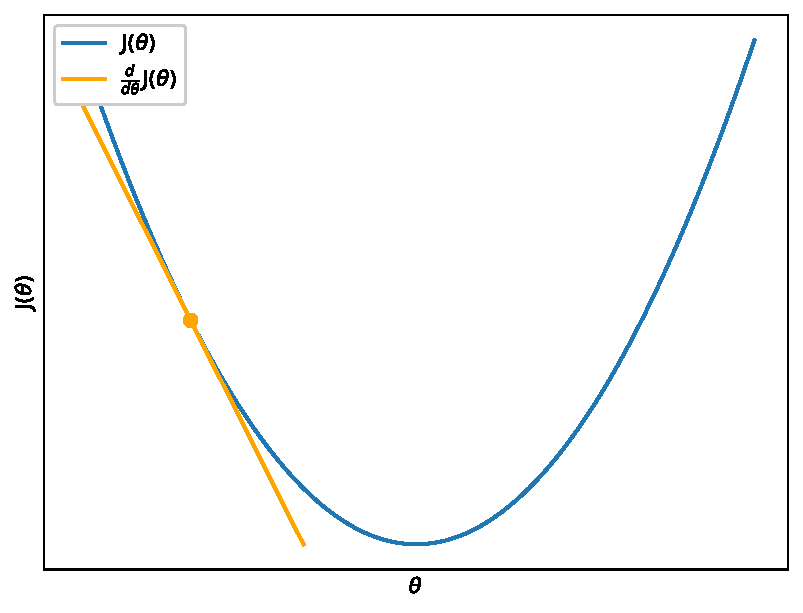
\includegraphics[width=0.5\textwidth]{chapters/NeuralNets/figures/1D-Loss.pdf}
    \fonte{From the author (2021)}
    \label{fig:1d_loss}
\end{figure}

Consider that the network initially starts with the parameter $\theta_0$ and loss $J_0$ at the dot shown in \autoref{fig:1d_loss}. To reduce the loss is to update the parameter $\theta$ in the opposite direction of the surface derivative. This can be shown by the following derivation.
\begin{align}
    J_0 + \Delta J & < J_0 \nonumber \\
    J_0 + \Delta\theta \frac{dJ}{d\theta} & < J_0 \nonumber \\
    \Delta\theta \frac{dJ}{d\theta} & < 0 \nonumber \\
    \sign(\Delta\theta) & = -\sign\left( \frac{dJ}{d\theta} \right) \label{eq:delta_theta_sign}
\end{align}

This derivation above only holds true for small values of $\Delta\theta$, since the derivative is calculated on infinitesimal small values, bigger changes run the risk of overshooting the region where the derivative approximation is reasonable.
\autoref{eq:delta_theta_sign} shows that the parameter change must be in the opposite direction of the change in the loss, the parameter updates can then be written as shown in \autoref{eq:1d_update}.
\begin{equation} \label{eq:1d_update}
    \theta_{i+1} = \theta_{i} + \Delta\theta = \theta_{i} - \eta \frac{dJ}{d\theta}
\end{equation}

\glsunset{learning_rate}
The value \gls{learning_rate} is a positive real number that determines how big are the steps taken when updating the parameters. This value is also a hyperparameter and is called the \textit{learning rate} of the network. A small learning rate is more precise but can make the training very slow, while bigger values are faster, but run the risk of overshooting and zigzaging around the target, or even worse, diverging and never reaching the result. \autoref{fig:1d_weight_update} shows how an initial parameter value is updated when using different values for $\eta$, it can be seen that there is a critical value $\eta_{crit}$ that is able to minimize the loss in a single step, while smaller and bigger values will converge to the minimum in multiple steps, and much bigger values will diverge.
\begin{figure}
    \centering
    \caption{Parameter updates for 1D loss surface in function of learning rate}
    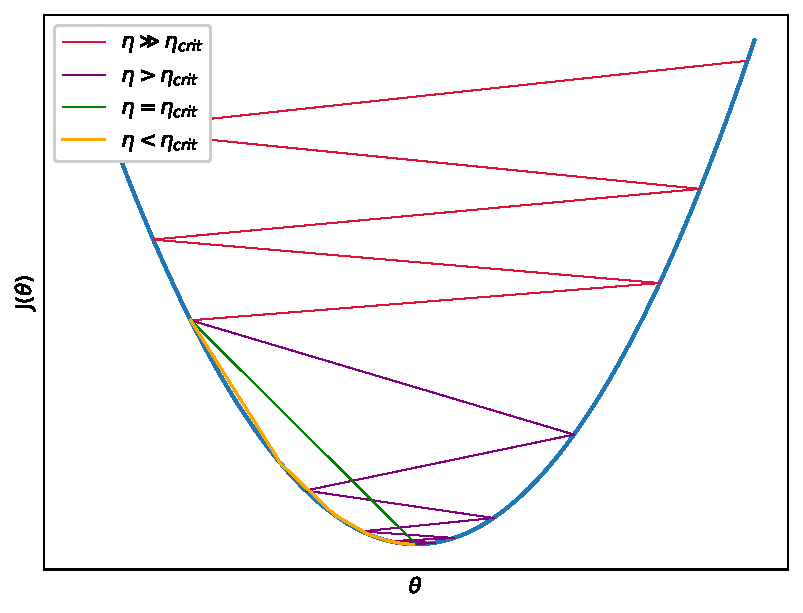
\includegraphics[width=0.5\textwidth]{chapters/NeuralNets/figures/1D-Weight-Update.pdf}
    \fonte{From the author (2021)}
    \label{fig:1d_weight_update}
\end{figure}

For one dimension it is relatively simple to find the critical learning rate, but for very high dimensional problems this is unfeasible or even impossible since a critical value for one parameter is not necessarily the same for all other parameters.

In practice, it is usually necessary to experiment with some values in order to find what best suits the loss surface of the problem, it is also common to employ some sort of dynamic update that slowly reduces the learning rate, allowing for big steps in the beginning while being more precise towards the end.


\subsection{Gradient Descent} \label{sub:gradient_descent}
The same derivation used to obtain \autoref{eq:delta_theta_sign} can be applied to generalize the minimization procedure to higher dimensional parameter spaces, the only difference is to consider the partial derivatives for each parameter. Doing this would reveal that, like in the 1-dimensional case, the change in a parameter $\theta^{(j)}$ must be in the opposite direction of the partial derivative of the loss with respect to this parameter. The parameter update would then be given by \autoref{eq:parameter_update}.
\begin{equation} \label{eq:parameter_update}
    \theta_{i+1}^{(j)} = \theta_{i}^{(j)} - \eta \frac{\partial J}{\partial \theta^{(j)}}
\end{equation}

There is however another way to look at these updates. Recall that the gradient of any scalar function is a vector field composed of all it's partial derivatives, so the gradient of the loss function is the vector field given by \autoref{eq:gradient}.
\begin{equation} \label{eq:gradient}
    \renewcommand{\arraystretch}{1.2}
    \nabla_{\bm{\theta}} J = \begin{bmatrix}
        \frac{\partial J}{\partial\theta^{(1)}} \\
        \frac{\partial J}{\partial\theta^{(2)}} \\
        \vdots \\
        \frac{\partial J}{\partial\theta^{(n)}}
    \end{bmatrix}
\end{equation}

Also recall that for any function $f$, it's gradient at any given point is a vector that points towards the direction of steepest increase to the function at that point and the negative of this vector points to the steepest decrease \cite[Chapter~4.6]{calculusIII2016}. So the negative of the gradient $\nabla_{\bm{\theta}} J$ gives the direction to update all parameters in order to most reduce the loss function, this is what was being shown element-wise in \autoref{eq:parameter_update}. By grouping the derivatives it is possible to write the parameter updates in a much cleaner way.
\begin{equation} \label{eq:gradient_descent}
    \bm{\theta}_{i+1} = \bm{\theta}_{i} - \eta \nabla_{\bm{\theta}} J(\bm{\theta}_i)
\end{equation}

By repeating the process of calculating the gradient of the loss function and then updating all the network's parameters (given a sufficiently small learning rate), then eventually all parameters will converge to values that minimize the loss function. This is what is referred to as \textit{learning} in a neural network and this iterative process is called \textit{Gradient Descent}, since the steps are taken using the gradient in order to decrease the loss function \textbf{--} for maximization, the only difference is to update in the positive direction of the gradient and this is called \textit{Gradient Ascent}.

One important thing that was left unmentioned is the fact that this algorithm will almost surely converge to a local minimum in the loss surface instead of the global minimum. In the example shown for the 1-dimensional case the surface was very simple, with a single minimum value to converge, but even in these very simple cases it is possible to find surfaces much more complex (e.g. the curve $y = x + 2\sin x$ has infinitely many local minima but no global minimum). For the very high dimensional spaces and very complex geometries of the loss surfaces in neural networks, there will be many valleys where gradient descent will converge, but rarely those will be the optimal solution. The local minimum found will depend on the starting point in parameter space, and there is usually no better to way than just randomly selecting a point\footnote{
    This does not mean that the starting values are picked without any rhyme or reason, the starting point can have a huge impact on the network and it is very important to choose good values. However, initialization techniques are concerned with finding a random distribution with the right values of mean and variance to sample from. The point here is explicitly about the random nature of the starting point and not that this nature has no thought behind it.
}.

So if gradient descent will almost never reach the optimal solution, why would anyone use it? How can someone make sure that the local minimum found is good enough for the problem? Or if someone is trying to build a neural network and the results are not being good, how can this person know if this is caused by a legitimate problem on the network or the dataset, instead of simply being the fact that the training process was unlucky and found a bad local minimum? And perhaps most important, how is it possible that neural networks are achieving so much ground-breaking results while relying on gradient descent to learn?

This is indeed a worry that many researchers in the field have, but there are many options to combat this problem, it can be cited regularization techniques (e.g. $\ell_1$ and $\ell_2$ norms \textbf{--} see \autoref{sub:regularization}) and optimizers (e.g. \glsunset{SGD}\gls{SGD}, momentum, RMSProp, \glsunset{Adam}\gls{Adam} \textbf{--} see \autoref{sub:optimizers}) as examples. 

Besides that, \textcite{lossSurfaces2014} argue that global minimum are not necessarily the best option, since they have a high chance of overfitting to the data (see \autoref{sub:overfitting}), they also empirically verify that for big enough neural networks most local minima are very similar to one another and have high quality. Their conclusion is that in practice it is not worth to strive for the global minimum, given that for large networks local minima have high quality and may even generalize better to unseen data.

\section{Backpropagation} \label{sec:backpropagation}
Last section showed how learning in a neural network is a minimization problem on the loss function and that it is solved by repeatedly updating the network's parameters using the gradient of the loss. But how exactly is the gradient calculated? The loss function is a surface in very high dimensions, calculated by averaging some distance function between the network's output and the true output for all inputs on the dataset; and the output of the network is a mapping calculated by passing the input through possible thousands, millions, or more units, where each one can apply a nonlinearity to it's output. In summary, the loss surface is extremely complex and the same should be expected for it's gradient.

To make it simpler to understand how the gradient is calculated, the procedure will be shown only for the weights and biases parameters, since those are present in practically all neural networks (although sometimes the bias is omitted in some units). This section will suppose a neural network with $L+1$ layers, where layer $0$ is the input, layer $L$ is the output and values in between are hidden layers.

Essentially, calculating the gradients consists of a smart application of the chain rule of calculus. Recall that the chain rule is a way of calculating the derivative of composite functions, this means that for a function $y$ that depends on $t$, and $t$ that depends on $x$, then the chain rule allows for calculating the derivative of $y$ with respect to $x$ by compounding how $x$ changes $t$ and how $t$ changes $y$. For the case of single variable functions the chain rule is given by \autoref{eq:chain_rule} \cite[p. 406]{calculusIII2016}.
\begin{equation} \label{eq:chain_rule}
    \frac{dy}{dx} = \frac{dy}{dt} \frac{dt}{dx}
\end{equation}

But for the case of neural networks, the loss function is dependent on all the activations of the output layer, and those are dependent on their weights, biases, and possibly other parameters, besides being dependent on activations of the previous layer. So it is necessary to use the multi-variable generalization of the chain rule shown in \autoref{eq:chain_rule_general} \cite[p. 412]{calculusIII2016}, here it is necessary to compound the effect of $x$ for all the variables $(t_0, t_1, \dots t_n)$ that $y$ is dependent on.
\begin{equation} \label{eq:chain_rule_general}
    \frac{\partial y}{\partial x} = \sum_{i}^{n}{\frac{\partial y}{\partial t_i} \frac{\partial t_i}{\partial x}}
\end{equation}

Having the chain rule in mind, it is also useful to define an additional term $\delta$ that represents the partial derivative of the loss with respect to the weighted input of a unit. For unit $i$ on layer $l$ this term is given by \autoref{eq:neuron_delta}.
\begin{equation} \label{eq:neuron_delta}
    \delta_{i}^{(l)} = \frac{\partial J}{\partial z_i^{(l)}}
\end{equation}

And lastly, note that by differentiating Equations \ref{eq:activation_again} and \ref{eq:dense_weighted_input}, the following relations are obtained.
\begin{equation*}
    \frac{\partial z_i^{(l+1)}}{\partial a_i^{(l)}} = w_{ij}^{(l+1)}
    \qquad
    \qquad
    \frac{\partial z_i^{(l)}}{\partial b_i^{(l)}} = 1
    \qquad \qquad
    \frac{\partial z_i^{(l)}}{\partial w_{ij}^{(l)}} = a_j^{(l-1)}
    \\[2pt]
\end{equation*}

The main idea of this algorithm is to derive $\delta$ for all layers, then use these values to calculate the gradient terms for all parameters, the first step is to calculate $\delta$ in the last layer. For the following derivation, consider $\hat{\bm{y}}$ as the network output, and notice that it is the same as the activations of the output layer $\bm{a}^{(L)}$. By using this knowledge, \autoref{eq:delta_last_layer} is derived as follows.
\begin{align}
    \frac{\partial J}{\partial z_i^{(L)}} = \delta_{i}^{(L)} &=
    \frac{\partial J}{\partial \hat{y_i}} \frac{\partial \hat{y_i}}{\partial z_i^{(L)}} \nonumber \\[10pt]
    %
    &= \frac{\partial J}{\partial \hat{y_i}} \frac{\partial a_i^{(L)}}{\partial z_i^{(L)}} \nonumber \\[10pt]
    %
    &= \frac{\partial J}{\partial \hat{y_i}} \frac{\partial}{\partial z_i^{(L)}} {f\left(z_i^{(L)}\right)} \nonumber \\[10pt]
    %
    \delta_{i}^{(L)} &= \frac{\partial J}{\partial \hat{y_i}} f'\left(z_i^{(L)}\right) \label{eq:delta_last_layer}
\end{align}

Recall that the loss function $J$ and activation function $f$ should both be continuous and differentiable, and since they are chosen when building the network their derivatives are known. The values $\hat{y_i}$ and $z_i^{(L)}$ are also known since they are calculated by the network and can be easily stored during training. This means that \autoref{eq:delta_last_layer} can be used to calculate all $\delta$ values in the last layer.

By using \autoref{eq:delta_last_layer} it is also possible to find an expression to calculate all the other $\delta$ values, the following derivation shows how this can be done by writing $\delta^{(l)}$ in terms of $\delta^{(l+1)}$ as shown in \autoref{eq:delta_hidden_layer}.
\begin{align}
    \frac{\partial J}{\partial z_j^{(l)}} = \delta_j^{(l)} &= \sum_{i}{
        \frac{\partial J}{\partial z_i^{(l+1)}}
        \frac{\partial z_i^{(l+1)}}{\partial a_j^{(l)}}
        \frac{\partial a_j^{(l)}}{\partial z_j^{(l)}}
    } \nonumber \\[10pt]
    %
    &= \sum_{i}{
        \delta_i^{(l+1)}
        \frac{\partial z_i^{(l+1)}}{\partial a_j^{(l)}}
        \frac{\partial a_j^{(l)}}{\partial z_j^{(l)}}
    } \nonumber \\[10pt]
    %
    &= \sum_{i}{
        \delta_i^{(l+1)}
        w_{ij}^{(l+1)}
        \frac{\partial a_j^{(l)}}{\partial z_j^{(l)}}
    } \nonumber \\[10pt]
    %
    \delta_j^{(l)} &= \sum_{i}{
        \delta_i^{(l+1)}
        w_{ij}^{(l+1)}
        f'\left( z_j^{(l)} \right)
    } \label{eq:delta_hidden_layer}
    %
\end{align}

Notice how the algorithm works, first the input is feedforwarded through the network to obtain the output $\hat{\bm{y}}$, this value is used to calculate $\delta^{(L)}$, that is then \textit{backpropagated} through the network in order to calculate $\delta^{(l)}$ for all previous layers. This process gives the name \textit{Backpropagation} to the algorithm.

Now for calculating the gradients using $\delta$. Notice that for this case, where only the weights and biases are being considered, the gradient depends on the change $\partial J$ with respect to $\partial b_i^{(l)}$ and $\partial w_{ij}^{(l)}$ for all units and layers.

The following derivation applies the chain rule to obtain the relation in \autoref{eq:gradient_bias} for the partial derivatives of the loss with respect to all the biases parameters.
\begin{align}
    \frac{\partial J}{\partial b_i^{(l)}} &= \sum_{k}{
        \frac{\partial J}{\partial z_k^{(l)}}
        \frac{\partial z_k^{(l)}}{\partial b_i^{(l)}}
    } \nonumber \\
    %
    &= \frac{\partial J}{\partial z_i^{(l)}} \frac{\partial z_i^{(l)}}{\partial b_i^{(l)}} + 
    \sum_{k \neq i}{
        \frac{\partial J}{\partial z_k^{(l)}}
        \cancelto{0}{\frac{\partial z_k^{(l)}}{\partial b_i^{(l)}}}
    } \nonumber \\[10pt]
    %
    &= \frac{\partial J}{\partial z_i^{(l)}} \nonumber \\[10pt]
    %
    \frac{\partial J}{\partial b_i^{(l)}} &= \delta_{i}^{(l)} \label{eq:gradient_bias}
\end{align}

The derivation for \autoref{eq:gradient_bias} first breaks the partial derivative of the cost in terms of the weighted inputs $\bm{z}^{(l)}$ in the layer where the bias is present. This is enough since the bias can not influence any previous layers and all influences in the next layers are already captured in the change $\partial J$ with respect to the weighted inputs $\partial z_k^{(l)}$. Since it is also known that the bias does not influence any other unit in the layer, the derivation could have been made directly without breaking the derivative into a sum of all the terms in the layer, but the whole process was shown here for completion sake.

A similar rationale can be used for the weight parameters, obtaining the relation seen in \autoref{eq:gradient_weight}.
\begin{align}
    \frac{\partial J}{\partial w_{ij}^{(l)}} &= \sum_{k}{
        \frac{\partial J}{\partial z_k^{(l)}}
        \frac{\partial z_k^{(l)}}{\partial w_{ij}^{(l)}}
    } \nonumber \\
    %
    &= \frac{\partial J}{\partial z_i^{(l)}} \frac{\partial z_i^{(l)}}{\partial w_{ij}^{(l)}} + 
    \sum_{k \neq i}{
        \frac{\partial J}{\partial z_k^{(l)}}
        \cancelto{0}{\frac{\partial z_k^{(l)}}{\partial w_{ij}^{(l)}}}
    } \nonumber \\[10pt]
    %
    &= \frac{\partial J}{\partial z_i^{(l)}} a_{j}^{(l-1)} \nonumber \\[10pt]
    %
    \frac{\partial J}{\partial w_{ij}^{(l)}} &= \delta_{i}^{(l)} a_{j}^{(l-1)} \label{eq:gradient_weight}
\end{align}


\autoref{eq:gradient_weight} was the last piece of the puzzle, together with Equations \ref{eq:delta_last_layer}, \ref{eq:delta_hidden_layer}, and \ref{eq:gradient_bias}, it can be applied to calculate the gradient for all parameters in the network, and this allows for gradient descent to update the parameters and minimize the loss function. From data to model, a complete procedure for a machine to learn by itself.

There are still some more concepts that will be briefly explored in the next section. One further detail to mention about backpropagation is the fact that the derivations in this section were only made for the weights and biases parameters, what about possible others? There are many different types of additional parameters, but the idea with backpropagation is that the $\delta$ values are already calculated for all the units in the network, any new parameter $\theta$ must simply have a correlation with some of these values in order to obtain $\partial J$ in terms of $\partial\theta$ and apply gradient descent for updates. Modern libraries and frameworks already abstract most of these calculations for the programmer via underlying procedures of automatic differentiation, for example, Tensorflow \cite{tensorflow2015} provides a \texttt{GradientTape} object to automatically watch and calculate the gradients for any desired parameter.

\section{Other concepts} \label{sec:other_NN_concepts}
This section will briefly describe some other concepts that are relevant to this document but not warrant a thorough explanation.

\subsection{Overfitting} \label{sub:overfitting}
One fundamental principle, not only for neural networks but many other machine learning techniques, is the idea of generalization. An algorithm that learned by training on some given data should be able to produce good results not only on this seen data, but also on similar and never before seen data. In the case of supervising learning problems for example, all the data is already labeled, there is no need to create a complex algorithm that can find these labels since the answer is already know. When teaching machines to think, the goal is not to make them memorize all the inputs and outputs, it is instead to make them learn how to abstract the data, to capture the fundamental patterns, and to interpret the input in a high level (e.g. seeing shapes, and objects instead of just pixels).

Since in the majority of cases the data available for training is only a fraction of the possible values expected for the problem, a machine learning algorithm must be able to use this relatively small amount of data to project how all the input space is distributed. This is as much a task for the algorithm as is for the dataset itself, the training data should contain enough samples to offer an accurate representation of how the input space is truly distributed. Ideally this data should be diverse enough to represent well the possible inputs (e.g. when training to differentiate between cats and dogs, the data should contain photos of both cats and dogs of multiple colors, in various angles, and with different poses) and it also should contain as much samples as possible\footnote{
    Although having too much representation for one region of the input space in relation with the others can introduce bias in the model. For example, \cite{networkBias2018} found that some gender classification systems had a significant higher error rates for dark skinned women (as high as 30\% higher than for white males) and that some facial analysis datasets underrepresented minorities in the samples. A similar problem happened to amazon, where an AI recruiting system was discriminating women for jobs since most of the resumes that it was trained on came from men \cite{amazonBias2018}. One proposed approach to combat this problem is to train another network to learn how the data is distributed and sample more from underrepresented data \cite{debiasingVAE2019}.
}.

\begin{figure} [hbt]
    \centering
    \caption{Visual representation of a learning algorithm fit to noisy data}
    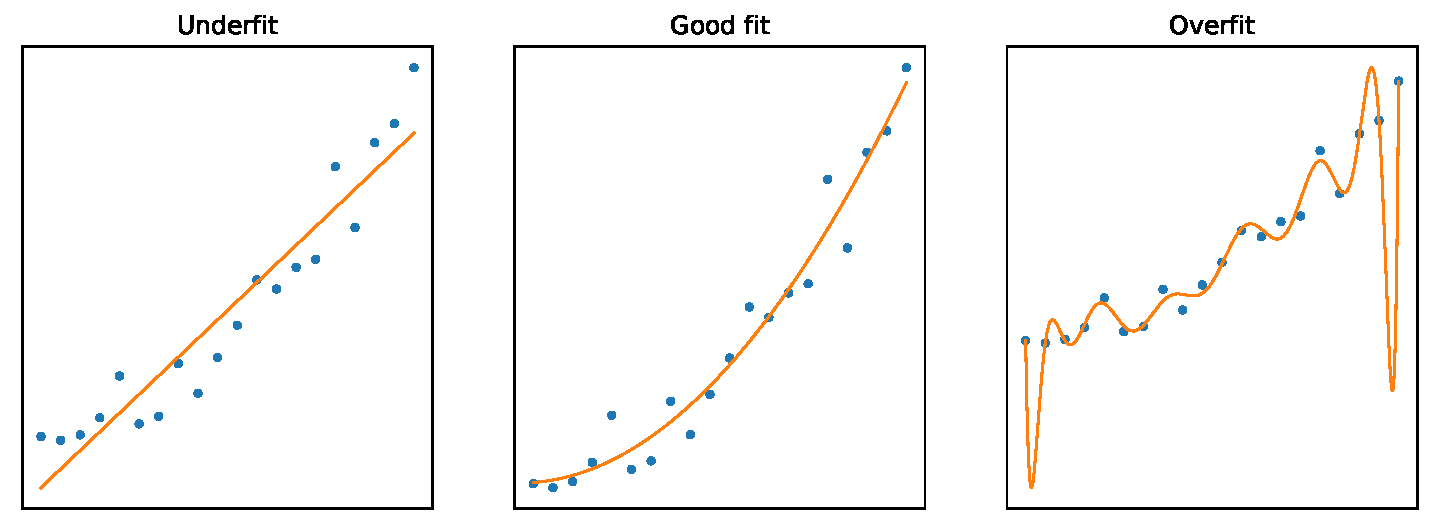
\includegraphics[width=0.8\textwidth]{chapters/NeuralNets/figures/fitting.pdf}
    \fonte{From the author (2021)}
    \label{fig:fitting}
\end{figure}
When the dataset is insufficient or the learning algorithm is not capable enough, the final model will only partially represent the data, but will not be able to capture all the details of the representation; this is called \textit{Underfitting}, the model was not able to fully represent the structure of the problem. In the other hand, the algorithm can also go to the opposite extreme and learn the dataset too well, this means that it will pick up particularities of the training data that don't generalize to the whole input distribution; this is called \textit{Overfitting} and it is facilitated by small datasets that don't represent much variety (noise in a sample has more influence in the signal to noise ratio of the whole dataset), or by networks that have too many degrees of freedom. \autoref{fig:fitting} visually represents the different fits for a 1-dimensional case.

Overfitting is however so common that it is almost natural to expect its appearance, it is one of the most prevalent problems in machine learning and there are many existing techniques to avoid it. The first step is to have a good quality dataset, data augmentation methods can be used to easily multiply the number of samples without much downsides. In the algorithmic side, next subsection will discuss regularization and how it can combat overfitting among other things.

\subsection{Regularization} \label{sub:regularization}
According to \cite[p. 117]{deepLearningBook2016}: ``\textit{Regularization is any modification we make to a learning algorithm that is intended to reduce its generalization error but not its training error}''. This is a general definition that encompasses many different techniques for regularization, but for this document it will suffice to describe only dropout and the $\ell_1$ and $\ell_2$ norms.

\subsubsection{L1 and L2 norms}
Since one of the reasons overfitting happens is because the models are given a large number of free parameters to adjust to the dataset (worth mentioning again the 175 billion parameters present in GPT-3 \cite{gpt3_2020}), then a common way of reducing overfitting is to limit the choice of parameters by adding a penalization term $\Omega(\bm{\theta})$ to the loss function as shown in \autoref{eq:regularization_penalty} \cite[p. 226]{deepLearningBook2016}.
\begin{equation} \label{eq:regularization_penalty}
    \tilde{J}(\bm{X}, \bm{\theta}) = J(\bm{X}, \bm{\theta}) + \lambda\Omega(\bm{\theta})
\end{equation}

The \gls{lambda} term is a positive hyperparameter that determines how much the penalty is relevant to the overall loss. For $\ell_1$ and $\ell_2$ norms, $\Omega(\bm{\theta})$ will be the respective norm of the $\bm{\theta}$ parameters. The $\ell_2$ norm is the standard distance in euclidean space, so for this norm the penalty term is given by \autoref{eq:l2_norm}.
\begin{equation} \label{eq:l2_norm}
    \ell_2(\bm{\theta}) = \|\bm{\theta}\|_2 = \sqrt{\theta_0^2 + \theta_1^2 + \dots + \theta_n^2}
\end{equation}

For the $\ell_1$ norm, the value calculated is what is called the Manhattan distance or taxicab distance \cite[p. 102]{dataDrivenScience2019} and is calculated as shown is \autoref{eq:l1_norm}
\begin{equation} \label{eq:l1_norm}
    \ell_1(\bm{\theta}) = \|\bm{\theta}\|_1 =  |\theta_0| + |\theta_1| + \dots + |\theta_n|
\end{equation}

Both norms will penalize large parameter values and the modified loss function in \autoref{eq:regularization_penalty} will make gradient descent favor solutions that use smaller parameters. The \gls{lambda} hyperparameter then determines how much to favor these simpler solutions.

A simple explanation on why smaller values would reduce overfitting can be given by considering the case of fitting a polynomial to some data. Consider the overfitting case seen before in \autoref{fig:fitting}, fitting a polynomial to reduce the square error on that noisy data results in a reasonable good approximation around the data points, but the curve suddenly changes directions in the extremes because of the terms with the highest powers in the polynomial. To make the curve fit the noisy data, a least squares approach will usually produce very high coefficients to balance the higher powers, this reduces the error but will almost never produce the true behaviour behind the data. Penalizing high coefficients with regularization is a way to force the solution to assume simpler values.

This is in no way a rigorous argument for regularization, but it can be used to have an intuition. The goal of this section is just to introduce the concept, regularization is an active area of research and a lot of support for it is based on empirical evidence, there is no complete theory to explain how and why it works so well \cite[chap. 3]{NN&DL2015}.

One last thing to mention is the fact that $\ell_1$ norm promotes sparsity in the parameters, this means that this approach will usually find solutions where multiple parameters will equal zero, larger values of \gls{lambda} will promote more sparse models.

\subsubsection{Dropout}
Since the local minimum reached by a training process will depend on the starting values for the parameters, one common way to increase the accuracy of a model is create an ensemble of different networks trained in the same dataset but with different starting points and/or architectures \cite[Chapter 6]{NN&DL2015}. The model output can then be a combination of the outputs of the ensemble, the combination could be majority voting, an average between outputs, or any other sensible function. This gives better results because it is not expected that randomly initialized networks would make the same mistakes in all situations \cite[p. 253]{deepLearningBook2016}.

Dropout is a technique that can be interpreted as a way to approximate an exponentially large ensemble of networks while using a single network and without needing to train more models \cite{dropout2012}. The idea behind it is that during training, when feedforwarding the input through the network, some units should have a probability $p$ of being dropped from the calculation, that is, their activations are set to zero.

The idea of removing units during calculation may sound counter-intuitive, but like the $\ell$ norms it is a way of restricting the learning process so that the network can't build very complex connections. By removing random units in each iteration, the network must be able to learn to represent the data even if a great number of units are removed, it no longer can expect that a combination of units will be present when evaluating the result and so it cannot depend on complex inter-correlations between units \cite{dropout2012}.

By dropping different units, dropout effectively trains the ensemble of all sub-networks of the base network. Typical dropout rates are 20\% for the input layer and 50\% for hidden layers \cite[p. 255, 257]{deepLearningBook2016}.

\subsection{Optimizers} \label{sub:optimizers}
Gradient descent has the theoretical basis for convergence, but it has big problems for use in practice. The first problem is that the whole training set must be averaged when calculating the loss $J(\bm{\theta})$, even for small datasets this is quite restrictive, for larger datasets containing hundreds of thousands or millions of samples this can make each iteration take an immense amount of time. This type of approach is commonly called Batch Gradient Descent.

Another problem is that, even if calculating the gradient was very fast, the simple parameter update (recall \autoref{eq:gradient_descent}) can become very slow, specially later in training. The point in parameter space can reach a region in the loss surface where the curvature is minimal, making the gradients very small; the updates could also jump around a valley in the loss surface, never reaching the local minimum \cite{momentumWorks2017}.

For calculating the gradients faster there is the approach called \glsreset{SGD}\gls{SGD}. There are several different methods for better traversing the loss surface, these are called optimizers. For the purposes of this document only the Momentum, RMSProp, and \gls{Adam} optimizers will be briefly explained.

\subsubsection{Stochastic Gradient Descent}
Instead of calculating the gradient $\nabla_{\bm{\theta}} J$ for all inputs in the dataset, \gls{SGD} instead approximates this value by calculating it for a single sample on the input. This makes the updates much faster, but will cause the updates to fluctuate heavily because of the gross approximation; this however can be beneficial since it can make the updates jump to potentially better local minima and it has been shown that, for small learning rates, \gls{SGD} will also converge \cite{optimizers2016}.

Another way to approximate the gradient is by calculating it only for a mini-batch of the dataset, that is, a subset of $m$ samples of the data. This is called Mini-batch Gradient Descent but is also more commonly referred to as \gls{SGD} as well. Using mini-batches instead of a single sample gives more stable updates while still being very fast, the values for $m$ usually fall between $50$ and $256$ \cite{optimizers2016}, but lower values are also common.

Another advantage of the stochastic approach is that the noise in the gradient approximation has an added regularization effect \cite[p. 5]{practical_gradient_recomendations2012}.

\subsubsection{Momentum, RMSProp, and Adam}
\glsreset{Adam}
The simple parameter update (\autoref{eq:gradient_descent}) for Gradient Descent has some problems that make it difficult to converge in practice. Some of the problems mentioned by \textcite{optimizers2016} are: that it is hard to choose a good value for the learning rate; only using a single learning rate can be insufficient; the parameters can get stuck in difficult regions of the loss surface, especially saddle points.

Between the many different approaches to combat this, one of the most popular that is also recommended when training \acp{GAN} \cite[p. 20, 27]{nipsGAN2017} is the \gls{Adam} optimizer. This optimizer is essentially a combination of Momentum and RMSProp, two other very popular optimizers.

Momentum, as the name suggests, is a way to give some inertia to the gradient updates, accelerating in the consistent directions while dampening oscillations. This technique has a strong theoretical basis and can give a quadratic speedup on many functions \cite{momentumWorks2017}. Momentum changes the parameter updates by adding a velocity term controlled by a new hyperparameter $\beta$ as shown in the following equations.
\begin{gather} \label{eq:momentum}
    \bm{m}_{i} = \beta \bm{m}_{i-1} + \nabla_{\bm{\theta}} J(\bm{\theta}_{i-1}) \\
    %
    \bm{\theta}_{i} = \bm{\theta}_{i-1} - \eta \bm{m}_{i}
\end{gather}

The RMSProp algorithm also tries to reinforce movement to the most relevant directions, it does this by keeping a exponentially moving average $v$ of the gradient accumulation \cite[303-304]{deepLearningBook2016}. It also introduces another $\beta$ hyperparameter and changes the updates as follows.
\begin{gather}
    \bm{v}_{i} = \beta \bm{v}_{i-1} + (1 - \beta)\nabla_{\bm{\theta}} J(\bm{\theta}_{i-1})^2 \\
    %
    \bm{\theta}_{i} = \bm{\theta}_{i-1} - \frac{\eta}{\sqrt{\bm{v}_{i} + \epsilon}} \nabla_{\bm{\theta}} J(\bm{\theta}_{i-1})
\end{gather}

Recall that although these equations are represented in vector form, all operation are performed element-wise. Finally for the \gls{Adam} algorithm, it can be seen as a combination of the two previous algorithms. It introduces two new hyperparameters $\beta_1$ and $\beta_2$ and the parameter updates work as follows \cite{adam2017}.
\begin{gather}
    \bm{m}_i = \beta_1 \bm{m}_{i-1} + (1 - \beta_1) \nabla_{\bm{\theta}} J(\bm{\theta}_{i-1}) \\[5pt]
    \bm{v}_i = \beta_2 \bm{v}_{i-1} + (1 - \beta_2) \nabla_{\bm{\theta}} J(\bm{\theta}_{i-1})^2 \\[5pt]
    \hat{\bm{m}_i} = \frac{\bm{m}_i}{1 - \beta_1^i} \\[5pt]
    \hat{\bm{v}_i} = \frac{\bm{v}_i}{1 - \beta_2^i} \\[5pt]
    \bm{\theta}_i = \bm{\theta}_{i-1} - \eta \frac{\hat{\bm{m}_i}}{\sqrt{\hat{\bm{v}_i} + \epsilon}}
\end{gather}

\textcite{adam2017} mentions that good default values for the hyperparameters are $\alpha = 0.001$, $\beta_1 = 0.9$, $\beta_2 = 0.999$ and $\epsilon = 10^{-8}$. The Tensorflow library \cite{tensorflow2015} follows this default, only changing $\epsilon$ to a order of magnitude higher, that is, $\epsilon = 10^{-7}$.

\subsection{Batch Normalization}
One important aspect in training neural networks is the distribution of the inputs for a layer. As mentioned in \autoref{subsub:sigmoid} about sigmoid, \textcite{efficientBackprop2012} showed that inputs that are not zero centered will have some bias effect on parameter updates, to avoid this the layer inputs should all be shifted to have a mean of zero; the authors also suggest to normalize all inputs in order to have the same covariance and, if possible, to have their values be uncorrelated. This should significantly speed up the learning process since the network will not have to adapt to a different distribution for every input.

Normalizing inputs is then an easy and effective way for better learning, therefore being a very commonly used technique that will also be used for the experiments proposed in this document.

However \textcite{batchnorm2015} note that for any layer in the network, the normalization idea for its inputs also applies; that is, any hidden layer feeding its output to the next layer can be considered as an input layer for a sub-network consisting of all the subsequent layers. Therefore, the same advantages for normalized inputs would be beneficial by normalizing hidden layer outputs.

Looking from the training perspective, each training iteration updates all parameters at the same time, but the gradient change in a layer gives the best change considering that all other layers remain constant \cite[p.313-314]{deepLearningBook2016}. In reality, changing the parameters of the previous layers will affect the distribution of inputs for the current layer, this constant change to the inputs of a layer resulting from changes to previous layers is what \textcite{batchnorm2015} call \textit{internal covariate shift}.

To address these issues \textcite{batchnorm2015} proposed a technique known as \gls{BN}, this method can be applied to any hidden layer and it consists of normalizing the layer inputs by the mean and variance of all the inputs in the current mini-batch. So, for a mini-batch $\mathcal{B}$ of size $m$ and inputs $(\bm{x}_1, \dots, \bm{x}_m)$, the normalized inputs $\hat{\bm{x}}_i$ are calculated using the mean $\bm{\mu}_{\mathcal{B}}$ and variance $\bm{\sigma}_{\mathcal{B}}$ of the batch. Equations \ref{eq:batch_mean}, \ref{eq:batch_variance}, and \ref{eq:batch_normalized_input} show how the mean, variance, and normalized inputs are calculated.
\begin{gather}
    \bm{\mu}_{\mathcal{B}} = \frac{1}{m}
    \sum_{i=1}^{m}{\bm{x}_i} \label{eq:batch_mean} \\[5pt]
    %
    \bm{\sigma_}{\mathcal{B}}^2 = \frac{1}{m}
    \sum_{i=1}^{m}{ \left( \bm{x}_i - \bm{\mu}_{\mathcal{B}} \right)^2 } \label{eq:batch_variance} \\[5pt]
    %
    \hat{\bm{x}}_i = \frac{ \bm{x}_i - \bm{\mu}_{\mathcal{B}} }
    { \sqrt{\bm{\sigma}_{\mathcal{B}}^2 + \epsilon} } \label{eq:batch_normalized_input}
\end{gather}

Note that these operations are applied element-wise for each component of the vectors, and again $\epsilon$ is used for numerical stability.

These operations result in the vectors $\hat{\bm{x}}_i$ having a mean of $0$ and variance of $1$ for each of their dimensions. However, by limiting the distribution to only these values also limits the representation power of the network \cite{batchnorm2015}, so the last step is to scale each one of the normalized activations by two new learnable parameters, $\gamma$ and $\beta$, unique for each activation, to obtain the transformed input $\bm{y}_i$ that can have any mean and variance. \autoref{eq:batch_transformed_input} shows how to scale the dimension $k$ of the normalized input $i$.
\begin{equation} \label{eq:batch_transformed_input}
    y_i^{(k)} = \gamma^{(k)} x_i^{(k)} + \beta^{(k)}
\end{equation}

This method has proven to be very powerful, with the original paper being able to reach the same accuracy as the, at the time state of the art image classification model, in 14 times less training iterations \cite{batchnorm2015}. The authors also cite a regularization effect of \gls{BN} that can reduce the need for other techniques like dropout.

When the authors originally proposed this method, they recommended applying the batch normalization operation directly to the weighted inputs of the network and only after apply the activation to the normalized values. However, since then \textcite{CaffeNetBench2017} empirically showed that applying \gls{BN} after the activation produces better results.

\subsection{Vanishing Gradients} \label{sub:vanishing_gradients}
Recall that for Equations \ref{eq:delta_last_layer} and \ref{eq:delta_hidden_layer} the $\delta$ term used to calculate the gradients, was directly dependent on the derivative of the activation function with relation to the weighted inputs $f'(\bm{z}^{(l)})$. Also note that the gradients are backpropagated through the network, which means that the $\delta$ values in a hidden layer are calculated from the $\delta$ in the next layer.

Consider now the case for a sigmoid or \gls{tanh} activation function which is applied to an weighted input far from zero, the activation in this case will be very close to the maximum or minimum value that the function can produce. When a unit outputs this kind of value it is said that it saturated, any slight deviation in the weighted input will barely have any difference in the activation value, in other words the derivative of the activation is close to zero.

Combining the points made in the last paragraphs it is possible to recognize a problem, when a unit saturates its gradient will be very small since the derivative of the activation is close to zero. Even worse than that is the fact that this small gradient will be backpropagated through the network, reducing the gradients of all previous layers. When many units saturate, this effect can compound, making the gradients for deeper layers very small and greatly reducing the training speed; this is the problem known as the \textit{Vanishing Gradients} problem.

One alternate case is when the gradients are high and compound to make the gradients in deeper layers become very high, making the steps too large and not converging to any local minima. This is called the \textit{Exploding Gradients} problem.

Both situations are undesirable and are specially worrying when trying to train very deep neural networks. Ideally the gradients should all be close to $1$ to make training consistent, but for saturating activation functions like sigmoid, there will usually be vanishing gradients \cite{NN&DL2015}. That is one of the main reasons to use non-saturating activation functions like \gls{ReLU} in the hidden layers of the network. Other common ways to combat this problem is to carefully initialize the network parameters and use small learning rates \cite{batchnorm2015}, these authors also suggest that \gls{BN} can be used on saturating units since it can reduce the chance that the input of the units will fall to the saturating regions.

